\chapter{Motivation} \label{chapter:MOTIVATION}

In the Lively Kernel, programmers can create applications by manipulating and composing graphical parts.
This chapter demonstrates the development of such parts and related recovery needs by example.


\section{Part Development By Example}

To exemplify how developers work directly on objects in the Lively Kernel, we will outline how a Lively Kernel user adds a new feature to the Lively Kernel's Object Editor.

\begin{figure}[h]
    \centering
    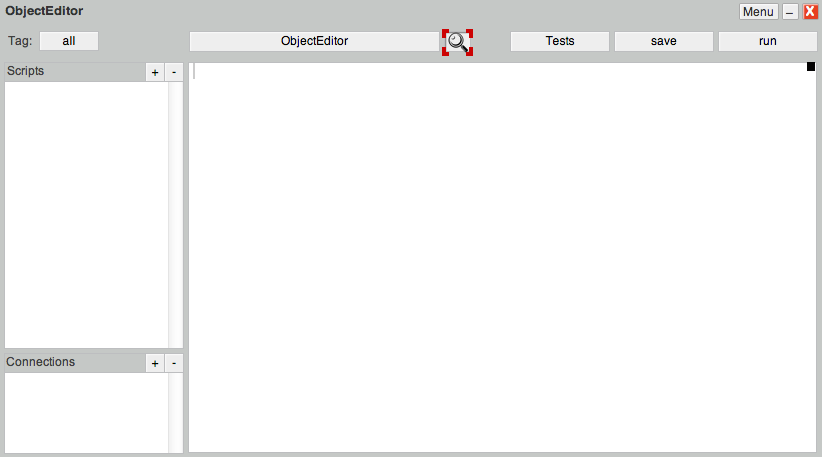
\includegraphics[width=0.8\textwidth]{figures/3_motivation/1_magnifierButton.png}
    \caption{The Object Editor with its magnifier button highlighted with a red outline.}
    \label{fig:MagnifierButton}
\end{figure}

The editor has been been developed by composing and editing graphical objects.
For this reason, the user does not adapt any source code modules to change the editor, but rather manipulates objects directly.

The feature the user adds in this example is a magnifier tool.
The magnifier tool helps in finding the editor's target, which is the object that the editor currently presents scripts for.
Adding the new feature requires to create a new button morph and to add the button to the editor, as shown in Figure~\ref{fig:MagnifierButton}.

The magnifier button has two features:
\begin{enumerate}
    \item When a programmer hovers over the button, the Object Editor's current target is highlighted with a rectangular overlay.
    \item When a programmer clicks the button, the current target selection is revoked and the programmer can select the new target of the editor.
\end{enumerate}

This example covers the first of the two features, which is also shown in Figure~\ref{fig:MagnifierBehavior} for an Object Editor currently targeting the character of a game.

\begin{figure}[h]
    \centering
    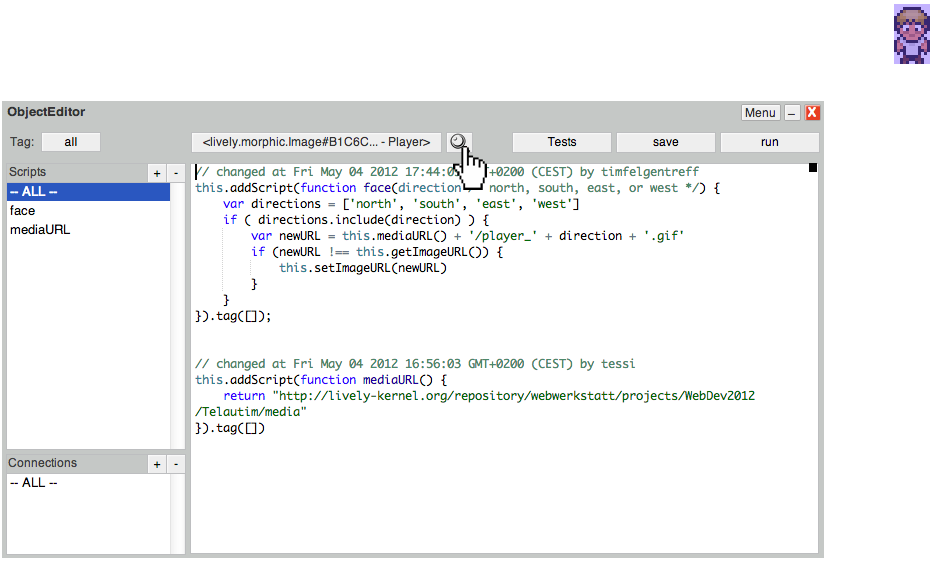
\includegraphics[width=0.8\textwidth]{figures/3_motivation/2_magnifierBehavior.png}
    \caption{Hovering the Object Editor's magnifier button highlights the current target object.}
    \label{fig:MagnifierBehavior}
\end{figure}

\paragraph{Manipulating the Button Morph}
Before implementing the button's behavior, the user first creates the button and manipulates its visual appearance.
Figure~\ref{fig:ButtonBuilding} shows the steps in which the button is manipulated.
A basic button, as visible in \circnum{1}, can be found in the Parts Bin repository.
In \circnum{2}, the user resizes the button and gives it a square extent using the \emph{Resize} halo button.
Next, the user loads an image showing a magnifier icon.
Using drag and drop the image is added to the button in \circnum{3}.
Dropping a morph onto another creates a parent-child relationship which connects the two morphs.
Moving the button around will then also move the image accordingly.
Finally, the users adds the result of these manipulations, visible in \circnum{4}, to the Object Editor.

\begin{figure}[h]
    \centering
    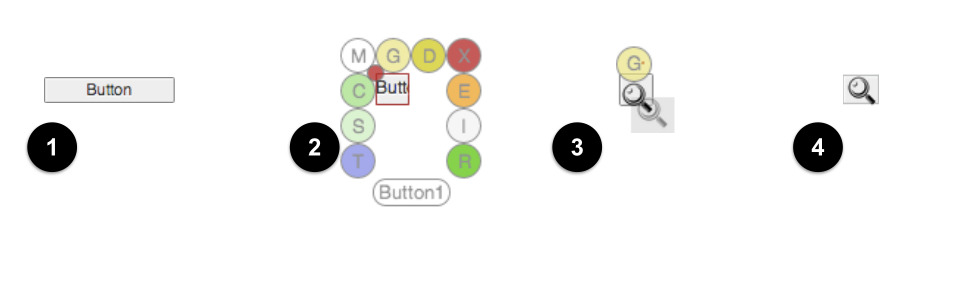
\includegraphics[width=0.8\textwidth]{figures/3_motivation/3_buildingTheButton.png}
    \caption{Directly manipulating a button morph.}
    \label{fig:ButtonBuilding}
\end{figure}

All these changes are made directly to the state of objects: the button morph, the magnifier image morph, and the editor morph.\\
When programmers edit parts in this way, they often see the effects of their actions immediately.
For example, when adding the new button to the Object Editor, the button is visible at all times.
Programmers do not need to run any code to see and test the result.

\paragraph{Scripting the Button Morph}
Next, the magnifier button needs its behavior.
The user adds scripts to the button that lay a translucent rectangle over the current target.
The implementation of this includes the following: 
\begin{itemize}
    \item The button holds a semitransparent rectangle morph.
    \item When the mouse enters the button (\lstinline{onMouseMove}), the button resizes and adds the rectangle to the world at the position of the target.
    \item When the mouse leaves the button (\lstinline{onMouseOut}), the button removes the rectangle from the world again.
\end{itemize}
 
When developing scripts with the Object Editor, the editor allows to evaluate code in the context of its target.
So, when programmers want to test a script or even just specific lines of code, they can often try the behavior directly for the actual target.


\section{Recovery Needs When Developing Parts}

While manipulating objects directly, developers might make changes that they later want to undo.

In the previous example the user could, for example, make \emph{accidental changes}:

\begin{itemize}
    \item \textbf{Accidental changes to state}: The user could accidentally grap and move a morph such as the new button and, thereby, change a carefully arranged layout. Similarly, meaningful state could also be lost when a morph as, for example, the editor with its new button is accidentally removed from the world.
    \item \textbf{Accidental changes to scripts}: The user could introduce a typographical error or accidentally remove a script. Moreover, editing a script could introduce an error or a decrease in performance.
\end{itemize}

Besides these accidental changes, also well-intentioned changes can turn out to be \emph{inappropriate changes}:

\begin{itemize}
    \item \textbf{Inappropriate changes through direct manipulation}: The user could make changes to the size, position, and colors of morphs to fine-tune the visual appearance of the editor's interface, only to decide later that a particular intermediate version was most appealing.
    \item \textbf{Inappropriate changes through scripts}: The user could make a mistake in a workspace snippet that is intended to manipulate morph properties programmatically. Such a snippet can change numerous properties of many objects, so re-establishing a previous state would be a laborious task.
\end{itemize}

\begin{figure}[h]
    \centering
    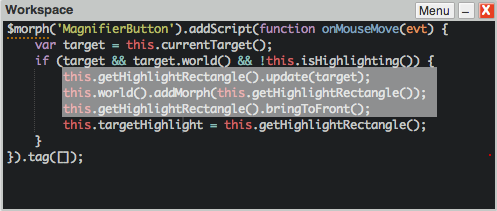
\includegraphics[width=0.7\textwidth]{figures/3_motivation/4_workspaceDoIt.png}
    \caption{The button's \lstinline{onMouseMove} script with a text selection.}
    \label{fig:onMouseOverScript}
\end{figure}

\paragraph{Explorative Script Evaluation}
Undesirable changes can also be introduced when a programmer explores the behavior of objects by evaluating scripts.
The Object Editor manipulates the scripts of a specific object and enables evaluating code directly for that target object.
While such evaluation might help to understand the effects of particular code, it might also change the state of objects.
For example, the user could be working on the button's \lstinline{onMouseMove} script and could evaluate a few lines of code to quickly test them.
These lines, as shown in Figure~\ref{fig:onMouseOverScript}, would add the rectangle to the editor's current target.
Evaluating just the selecting line would, however, not check the conditions usually above or set the state below these lines.
Thus, evaluating this selection allows to test the highlighting behavior but leaves the system in a state that it would not normally be in.

The examples show that there are many situations in which the user would want to undo actions.
In programming systems like the Lively Kernel, where programmers work on objects, the development state consists of the state of objects.
Changes are always made to the state of objects.
Functions are properties of objects and even classes and modules are objects.

For example, evaluating the text selection in Figure~\ref{fig:onMouseOverScript} changes the \lstinline{world} morph's state.
In particular, the \lstinline{world}'s collection of submorphs would be altered.
The world object has now one more submorph, as shown in Figure~\ref{fig:changedCharacter}.

\begin{figure}[h]
    \centering
    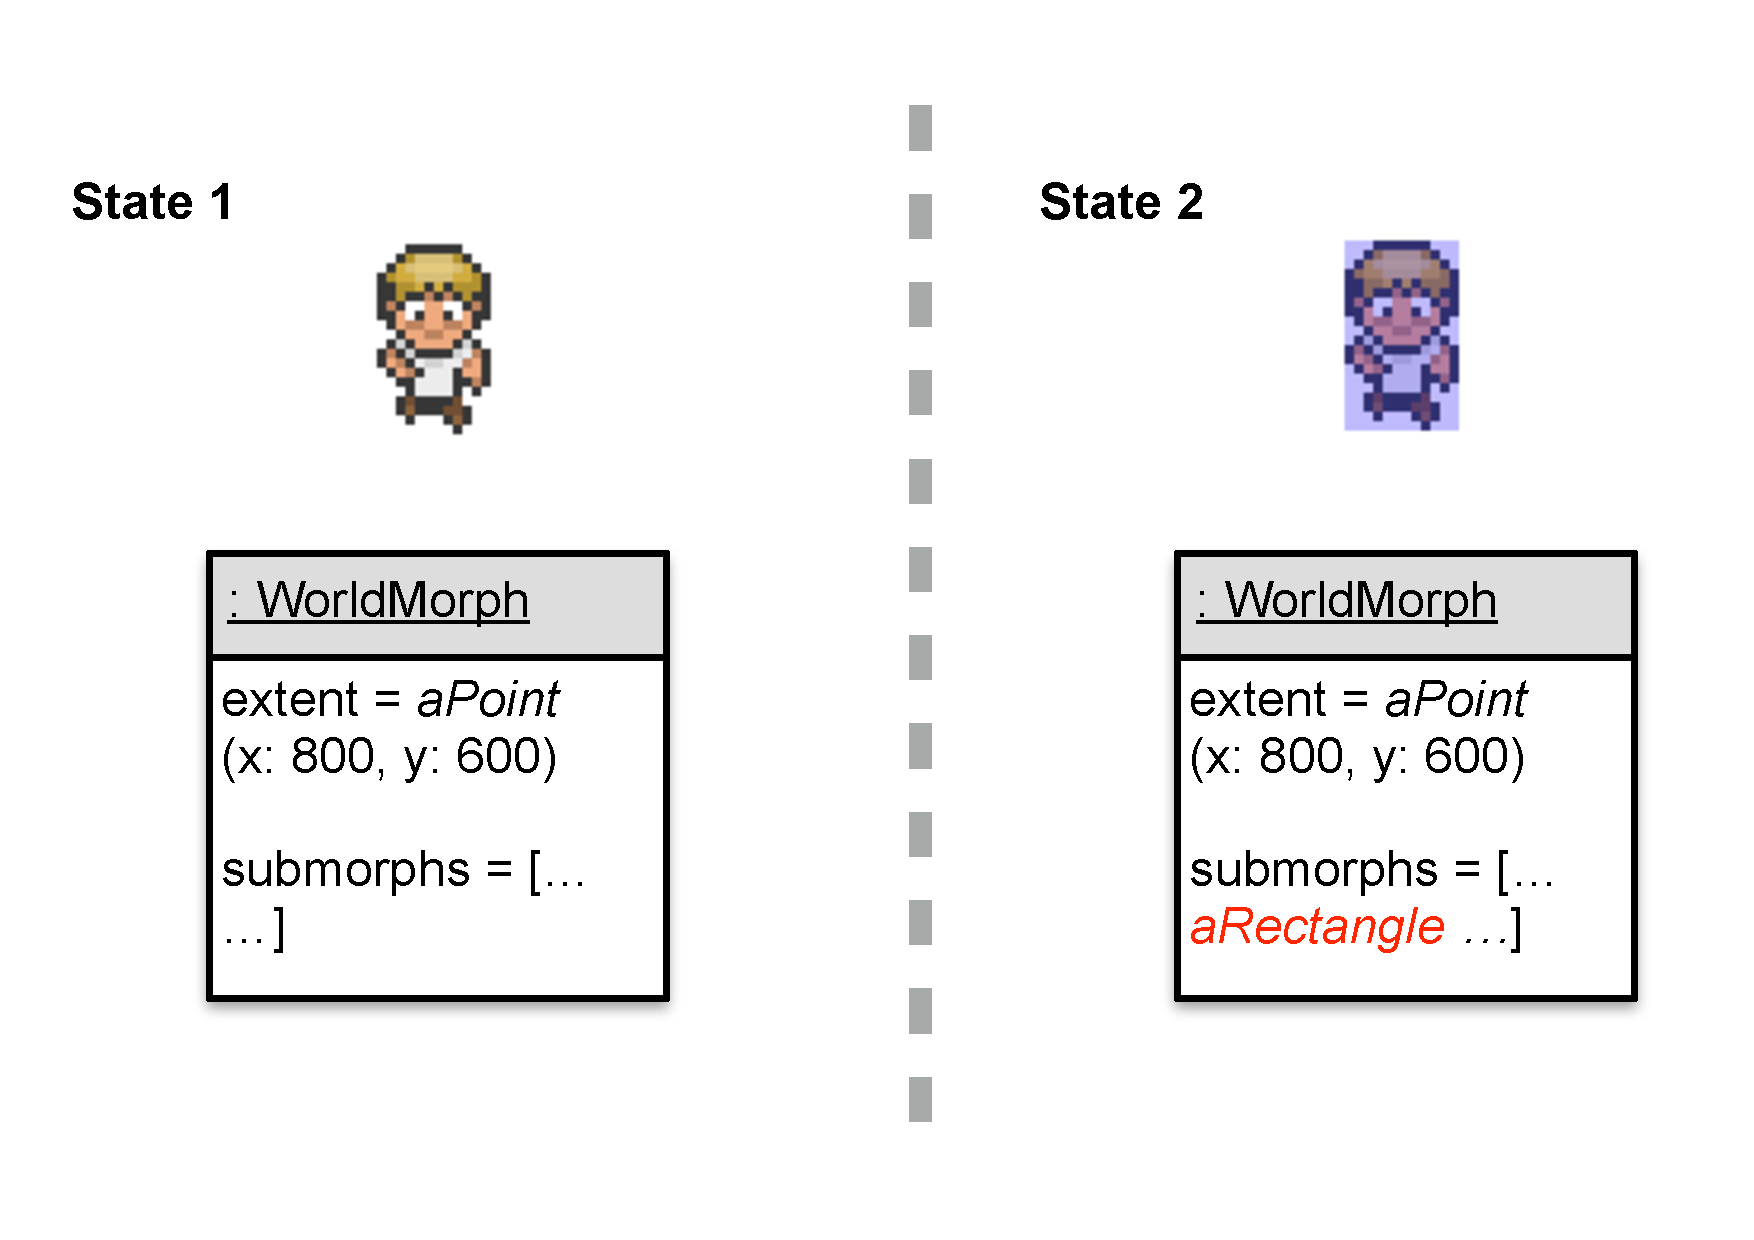
\includegraphics[width=0.6\textwidth]{figures/3_motivation/5_stateChanges.pdf}
    \caption{Adding a submorph changes the state of a morph.}
    \label{fig:changedCharacter}
\end{figure}

To undo the side-effect of the script and re-establish the previous situation, the change to the world object needs to be undone.
The worlds \lstinline{submorphs} property needs to be as it previously was.\\
When the state of all objects is preserved and can be re-established, previous system states can be recovered whenever recovery is necessary.
